\documentclass[12pt]{article}
\usepackage{amsmath}
\usepackage{booktabs}
\usepackage{listings}
\usepackage{graphicx}

\begin{document}

\title{Discrete Assignment-11.9.1-11}
\author{Hiba Muhammed \\
        EE23BTECH11026}
\maketitle

\section*{Problem Statement}
Write the first five terms in the sequence:
\[
\begin{aligned}
x_0 &= 3 \\
x_n &= 3x_{n-1} + 2 \quad \text{for } n > 1
\end{aligned}
\]

\section*{Solution}
\begin{table}[h]
  \centering
  \caption{Input Parameters: First Term and General Formula}
  \begin{tabular}{|c|c|}
    \hline
    \textbf{Term} & \textbf{Value} \\
    \hline
    \(x_0\) & 3 \\
    \(x_{n}\) & \(3x_{n-1} + 2\) for \(n > 1\) \\
    \hline
  \end{tabular}
\end{table}
Let's find the first 5 terms of the sequence:
\begin{align}
x_1 &= 3x_0 + 2 = 3 \times 3 + 2 = 11 \\x_2 &= 3x_1 + 2 = 3 \times 11 + 2 = 35 \\
x_3 &= 3x_2 + 2 = 3 \times 35 + 2 = 107 \\x_4 &= 3x_3 + 2 = 3 \times 107 + 2 = 323 \\
x_5 &= 3x_4 + 2 = 3 \times 323 + 2 = 971 
\end{align}

So, the next 5 terms of the sequence are \(11, 35, 107, 323, 971\).
\begin{figure}[h]
    \centering
    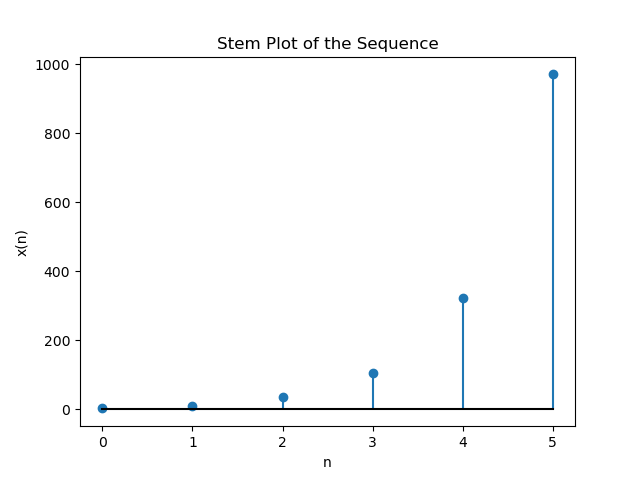
\includegraphics[width=0.7\linewidth]{11.9.1-11.png}
    \caption{Sequence plot generated from Python script.}
    \label{fig:sequence-plot}
\end{figure}

\end{document}

